\section{Prediction of values about the data}

Some basic and general goals were defined before starting this phase, with the idea of "doing more if it's possible". Basically the main purpose was the one of, after the previous analysis, predict some values and evaluate the quality of the results.
This prediction system was not defined with some specific requirements, so the first main problem was to find a reliable, accurated and user-friendly way to predict and display prediction of values.

Since the current dataset can be considered like a time series, in this phase we will develop the data prediction system using an ARIMA machine implemented in python.

The ARIMA machine can be configured with several configurations, it allows you to have more accurated results; so the first thing was to find the right configuration of the ARIMA machine of each single input which we are interested to forecast.

General steps of this experiment:
\begin{enumerate}
\item Test 112 different configurations for each single input that we would like to forecast and report the results with each MAPE (Mean Average Percentage Error) values.
\item Run the ARIMA Machine with the best configuration for that particular input, that means the configuration which displayed the lowest MAPE during the previous testing part.
\item Collect real 2017 values of each single input.
\item Display forecasted 2017 values and real 2017 values.
\end{enumerate}

During the implementation of this system have been implemented other 3 subsystems:
- Evaluating system: used for evaluate different configurations of ARIMA machine
- Testing system: used for display the result on a dataset already known
- Future prediction system: used for predict values in the future
	
\newpage
\subsection{Evaluating System}
\textbf{Goal:}\\ Used for evaluate different configurations of ARIMA machine

\textbf{Requirements:}\\
There are not strict requirements needed. The input dataset could be as long as you want.

\textbf{Code implementation:}\\
The most important part of the code about the Evaluating System is the following.\\
Basically the method ARIMA() allows to train a model based on historic values (history) and a specific order (p,d,q). After that it's possible to call the method forecast() through the trained method and having some predictions like result.
\begin{lstlisting}
model = ARIMA(history, order=arima_order)
model_fit = model.fit(disp=0)
yhat = model_fit.forecast()[0]
\end{lstlisting}

This system will provide 112 different ARIMA configurations results for each single input, and in particular it will display the best ARIMA configuration, that is the one with the lower MAPE.

\textbf{Results:}\\
The system will display the MAPE between real value and predicted values for each single tested ARIMA machine, in particular the configuration that gives the best result.
All these results have been reported in a document and then also displayed with a 3D graphic that allows to see the MAPE value for each different order in input.



\begin{figure}[H]
	\raggedleft
	\makebox[\textwidth][c]{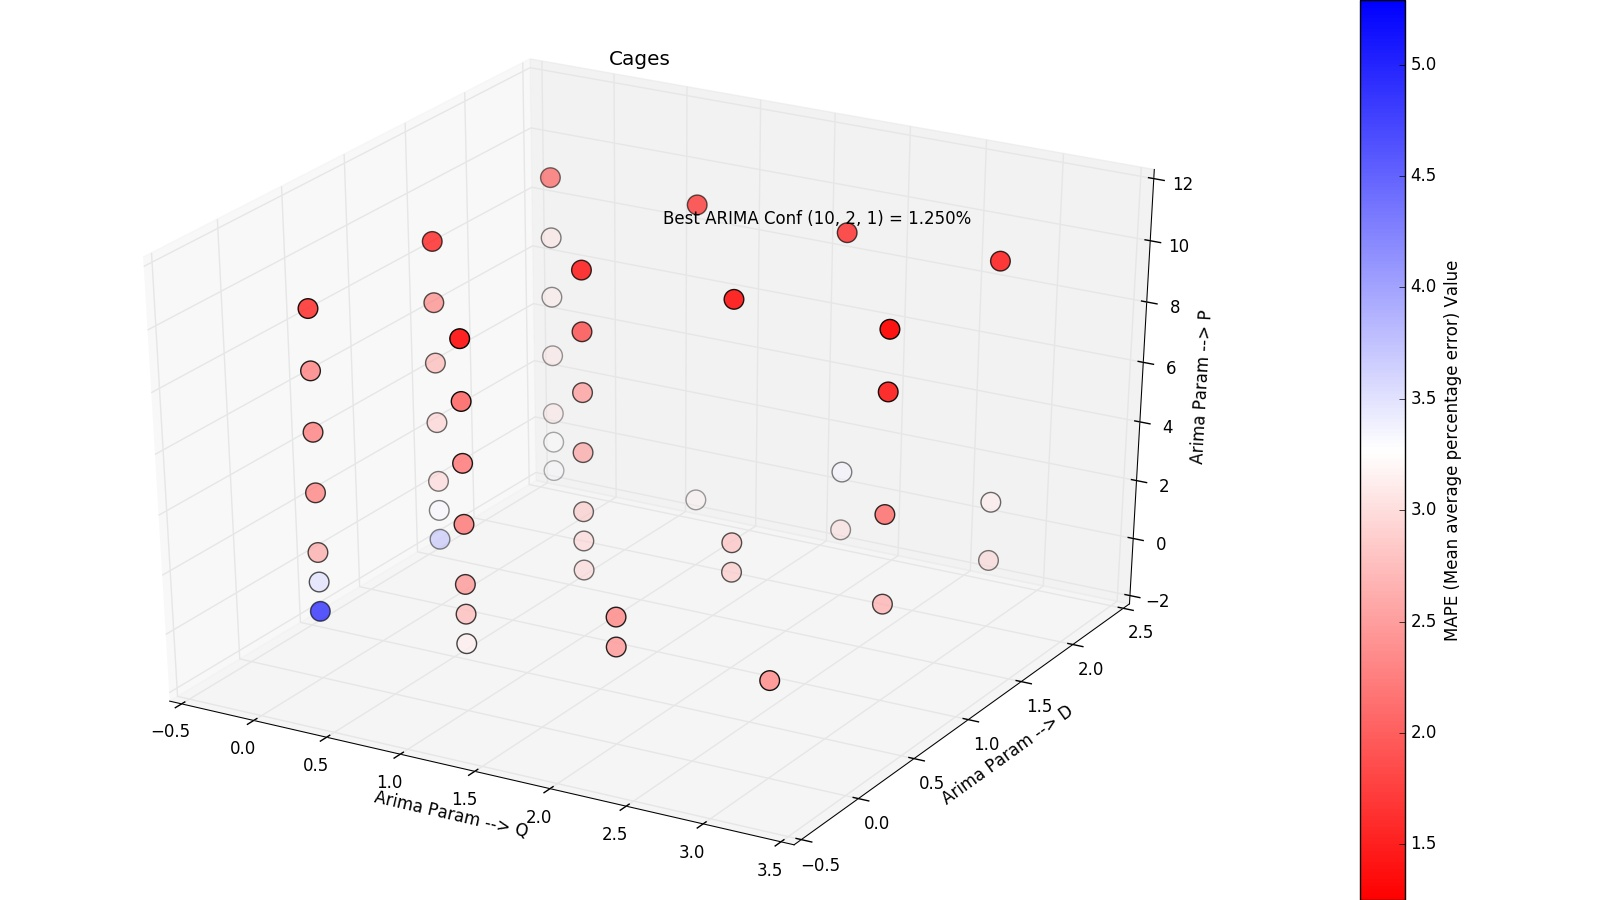
\includegraphics[width=0.7\textwidth]{Files/Cages_MAPE.jpg}}
    \caption{Graphic that displays different MAPE values for each ARIMA order.}
\end{figure}

 
 
\newpage
\subsection{Training System}
\textbf{Goal:}\\ Used for display the result on a dataset already known

\textbf{Requirements:}\\
Since this Traning System has been used mainly for train and test the current dataset, it need to have like input a dataset that follows the same format:
- Data content: 144 values, 1 value for each month from 2005 to 2016

\textbf{Code implementation:}\\
\begin{lstlisting}

\end{lstlisting}

\textbf{Results:}\\

\begin{figure}[H]
	\centering
    \makebox[\textwidth][c]{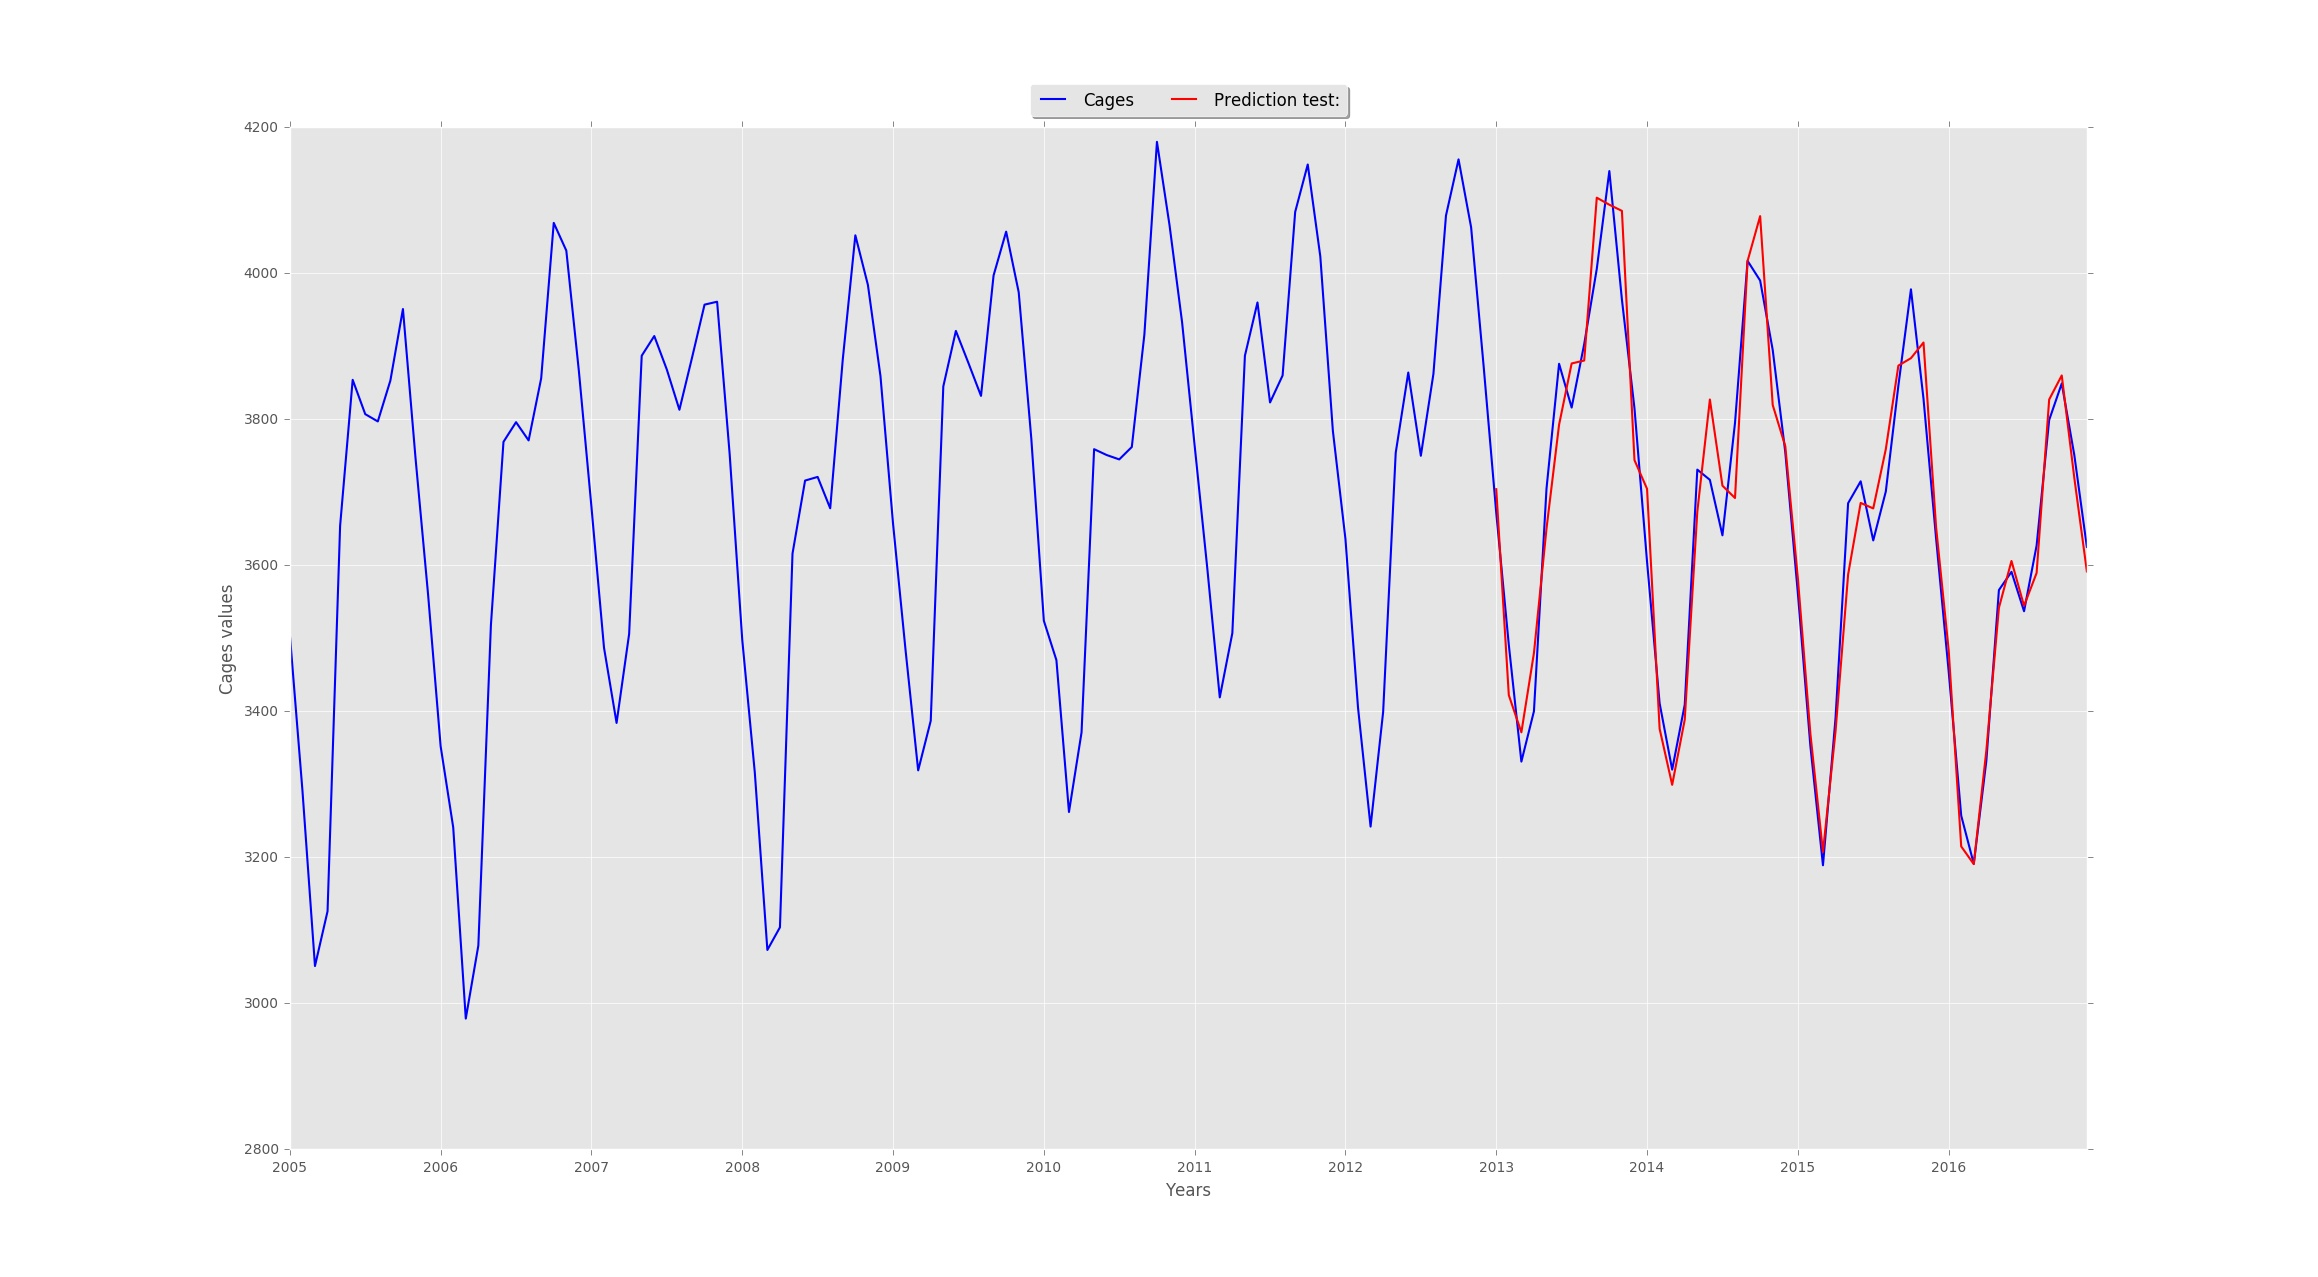
\includegraphics[width=1.5\textwidth]{Files/Cages_TRAIN.jpg}}
    \caption{Graphic that displays the predicted values from a particular ARIMA machine configuration and the historic real values.}
\end{figure}


\newpage
\subsection{Future Prediction System}
\textbf{Goal:}\\ Used for predict values in the future

\textbf{Requirements:}\\
- Input dataset:\\
- Data content:

\textbf{Code implementation:}\\
\begin{lstlisting}

\end{lstlisting}

\textbf{Results:}\\
\begin{figure}[H]
	\centering
    \makebox[\textwidth][c]{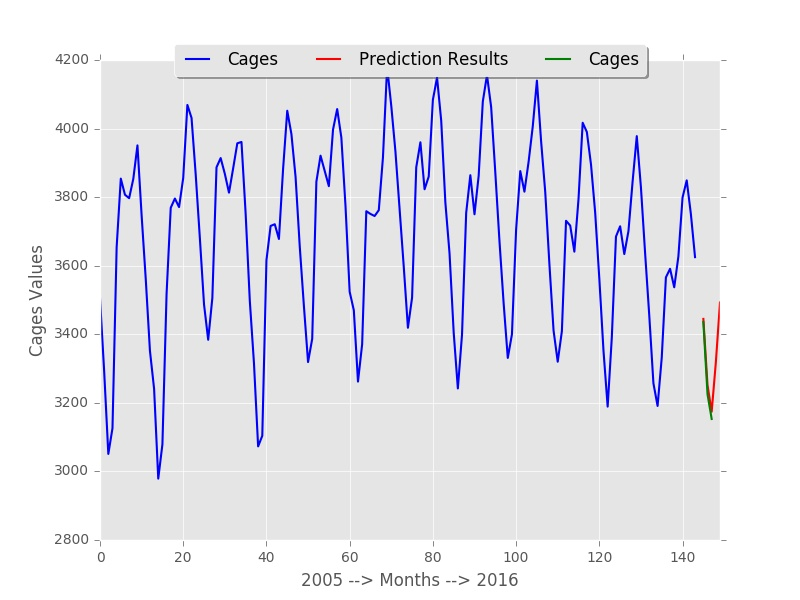
\includegraphics[width=1\textwidth]{Files/Cages_Predictions.jpg}}
    \caption{Graphic that display historic, future and predicted values of a input.}
\end{figure}

